% Nastaveni stranky
\documentclass[a4paper,oneside,13pt]{article}
\usepackage[utf8]{inputenc}
\usepackage[czech]{babel}
\usepackage[pdftex]{graphicx}
\usepackage{mathtools}
\usepackage{secdot}
\usepackage{pifont}
\usepackage{gensymb}
\usepackage{biblatex}
\usepackage{amsmath}
\usepackage{graphicx}
\addtolength{\textwidth}{3cm}
\addtolength{\hoffset}{-1cm}
\def\arraystretch{1.5}
\setlength{\jot}{10pt}
\setlength{\voffset}{-1.5cm}
\begin{document}
	\begin{titlepage}
	\centering
	%
\includegraphics[width=0.15\textwidth]{LOGO_VUT.PNG}\par\vspace{1cm}
	\vskip 5em
	{\scshape\LARGE VYSOKÉ UČENÍ TECHNICKÉ V BRNĚ \par}
	\vspace{1cm}
	{\scshape\Large Fakulta informačních technologií\par}
	\vspace{6cm}
	{\huge\bfseries Semestrální projekt do předmětu IEL\par}
	\vspace{0.5cm}
	{\Large Adam Sedláček $|$ xsedla1e\par}\vspace{0.5cm}
	{\large \today\par}\vspace{3cm}
	\begin{table}[ht]
		\begin{center}
			\begin{tabular}{|c|c|c|}
				\hline
				Úloha & Skupina & Výsledky \\
				\hline
				\RN{1}. & B & $U_{R1} = 67.2812V$, $I_{R1} =  0.1035A$ \\
				\hline
				\RN{2}. & B & $U_{R3} = 36.7500 V$, $I_{R3} = 0.1670A$ \\
				\hline
				\RN{3}. & H & $U_{R5} = 9.5504 V$, $I_{R5} = 0.3818A$ \\
				\hline
				\RN{4}. & B & $|U_{C1}| = 11.0060 V$, $\phi_{C1} = -0.7584 rad$ \\
				\hline
				\RN{5}. &  B & $U_{c}(t) = 40 - 32e^{-\frac{1}{200} t}$ \\
				\hline
			\end{tabular}
		\end{center}
	\end{table}
\end{titlepage}

%%%%%%%%%%%%%%%%%%%%%%%%%
%			PRVNI PRIKLAD			   %
%%%%%%%%%%%%%%%%%%%%%%%%%

	\newpage
	\section{Metoda zjednodušováním}
	
	Stanovte napětí $U_{R1}$ a proud $I_{R1}$. Použijte metodu postupného
	zjednodušování obvodu.

	\begin{table}[h]
		\begin{center}
			\begin{tabular}{|c|c|c|c|c|c|c|c|c|c|c|}
				\hline
				sk. & $U_1$ [$V$] & $U_2$ [$V$] & $R_{1}$ [$\Omega$] & $R_{2}$ [$\Omega$] & $R_{3}$ [$\Omega$] & $R_{4}$ [$\Omega$] & $R_{5}$ [$\Omega$] & $R_{6}$ [$\Omega$] & $R_{7}$ [$\Omega$] & $R_{8}$ [$\Omega$] \\
				\hline
				B & 95 & 115 & 650 & 730 & 340 & 330 & 410 & 830 & 340 & 220 \\
				\hline
			\end{tabular}
		\end{center}
	\end{table}
	
	\begin{figure}[h]
		\begin{center}
			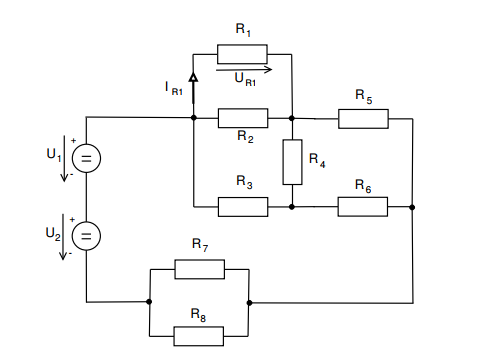
\includegraphics[width=14cm,keepaspectratio]{Odpory_1.PNG}
		\end{center}
	\end{figure}

	Zapojení zjednodušíme:
	\begin{eqnarray*}
		R_{12} & = & R_{1} || R_{2} = \frac{R_{1} *  R_{2}}{R_{1} +  R_{2}} = \frac{650*730}{650+730} = 343.8406 \Omega \\
		R_{78} & = & R_{7} || R_{8} = \frac{R_{7} *  R_{8}}{R_{7} +  R_{8}} = \frac{340*220}{340+220} = 133.5714 \Omega \\
	\end{eqnarray*}

	Nyní vzniklý trojuhelník $R_{4}$,  $R_{5}$,  $R_{6}$ převedeme na hvězdu:
	\begin{eqnarray*}
		R_{A} & = & \frac{R_{4} *  R_{5}}{R_{4} + R_{5} + R_{6}} = \frac{330 * 410}{330 + 410 + 830} = 86.1783 \Omega \\
		R_{A} & = & \frac{R_{4} *  R_{6}}{R_{4} + R_{5} + R_{6}} = \frac{330 * 830}{330 + 410 + 830} = 174.4586 \Omega \\
		R_{A} & = & \frac{R_{5} *  R_{6}}{R_{4} + R_{5} + R_{6}} = \frac{410 * 830}{330 + 410 + 830} = 216.7516 \Omega \\
	\end{eqnarray*}

	Zapojení následně ještě zjednodušíme:
	\begin{eqnarray*}
		R_{A12} & = & R_{12} + R_{A} = 343.8906 + 86.1783 = 430.0689 \Omega \\
		R_{B3} & = & R_{3} + R_{B} = 340 + 173.4586 = 514.4586 \Omega \\
		R_{AB123} & = & R_{B3} || R_{A12} = \frac{R_{B3} * R_{A12}}{R_{B3} +R_{A12}} = \frac{514.4586 * 430.0689}{514.4586 + 430.0689} = 234.2469 \Omega \\
	\end{eqnarray*}

	Nyní můžeme vypočítat $R_{ekv}$:
	\begin{eqnarray*}
		R_{ekv} & = & R_{AB123} + R_{C} + R_{78} = 234.2469 + 216.7516 + 133.5714 = 584.5699 \Omega \\
	\end{eqnarray*}

	Vypočteme proud:
	\begin{eqnarray*}
		I & = & \frac{U}{R_{ekv}} = \frac{210}{584.5699} = 0.3592A \\
	\end{eqnarray*}

	Teď můžeme vypočítat napětí na $R_{AB123}$:
	\begin{eqnarray*}
		U_{AB123} & = & I * R_{AB123} = 0.3592 * 234.2469 = 84.1415V \\
	\end{eqnarray*}

	Díky napětí, můžeme vypočítat proud $I_{A12}$:
	\begin{eqnarray*}
		I_{A12} & = & \frac{U_{AB123}}{R_{A12}} = \frac{84.1415}{430.0689} = 0.1956A \\
	\end{eqnarray*}

	Vypočteme napětí $U_{12}$:
	\begin{eqnarray*}
		U_{12} & = & I_{A12} * R_{12} = 0.1956 * 343.8406 = 67.2812V \\
	\end{eqnarray*}

	Teď už jen zbývá zjistit proud $I_{1}$:
	\begin{eqnarray*}
		I_{R1} & = & \frac{U_{12}}{R_{1}} = \frac{67.2812}{650} = 0.1035A \\
	\end{eqnarray*}

	Výsledné hodnoty jsou:
	\begin{eqnarray*}
		I_{R1} & = & 0.1035A \\
		U_{R1} & = & 67.2812V \\
	\end{eqnarray*}

%%%%%%%%%%%%%%%%%%%%%%%%%
%			DRUHY PRIKLAD			   %
%%%%%%%%%%%%%%%%%%%%%%%%%
	
	\newpage
	\section{Théveninuv teorém}
	
	Stanovte napětí $U_{R3}$ a proud $I_{R3}$. Použijte metodu Théveninovy věty.
	
	\begin{table}[h]
		\begin{center}
			\begin{tabular}{|c|c|c|c|c|c|c|}
				\hline
				sk. & $U_1$ [$V$] & $U_2$ [$V$] & $R_{1}$ [$\Omega$] & $R_{2}$ [$\Omega$] & $R_{3}$ [$\Omega$] & $R_{4}$ [$\Omega$]  \\
				\hline
				B & 100 & 50 & 310 & 610 & 220 & 570 \\
				\hline
			\end{tabular}
		\end{center}
	\end{table}
	
	\begin{figure}[h]
		\begin{center}
			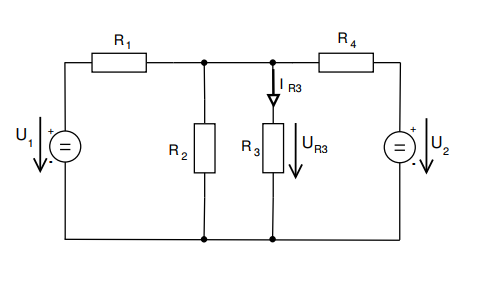
\includegraphics[width=12cm,keepaspectratio]{Thevenin_2.PNG}
		\end{center}
	\end{figure}
	
	Spojíme $R_{2}$ a $R_{3}$, které následně "vyjmeme" a zkratujeme zdroje:
	\begin{eqnarray*}
		R_{23} & = & R_{2} || R_{3} = \frac{R_{2} * R_{3}}{R_{2} + R_{3}} = \frac{610 * 220}{610 + 220} = 160.6867 \Omega \\
	\end{eqnarray*}

	Zjistíme $R_{i}$:
	\begin{eqnarray*}
		R_{i} & = & R_{1} || R_{4} = \frac{R_{1} * R_{4}}{R_{1} + R_{4}} = \frac{310 * 570}{310 + 570} = 200.7955 \Omega \\
	\end{eqnarray*}

	Zjistíme $U_{i}$:
	\begin{eqnarray*}
		0 & = & I_{x} * R_{1} + U_{i} - U_{1} \\
		I_{x} & = & \frac{U_{2} - U_{1}}{R_{1} + R_{4}} = \frac{50 - 100}{310 + 570} = -0.0568A \\
		U_{i} & = & U_{1} - I_{x} * R_{1} = 100 -17.6136 = 82.3864V \\ 
	\end{eqnarray*}

	Nyní můžeme vypočíst $I_{R23}$ a $U_{R23}$:
	\begin{eqnarray*}
		I_{R23} & = & \frac{U_{i}}{R_{i} + R_{23}} = \frac{82.3864}{200.7955 + 160.6867} = 0.2279A \\
		U_{R23} & = & R_{23} * I_{R23} = 160.6867 * 0.2279 = 36.75V \\
		I_{R3} & = & \frac{U_{R23}}{R_{3}} = \frac{36.75}{220} = 0.1670A \\
	\end{eqnarray*}
	
	Výsledné hodnoty jsou:
	\begin{eqnarray*}
		I_{R3} & = & 0.1670A \\
		U_{R3} & = & 36.75V \\
	\end{eqnarray*}

%%%%%%%%%%%%%%%%%%%%%%%%%
%			TRETI PRIKLAD			   %
%%%%%%%%%%%%%%%%%%%%%%%%%

	\newpage
	\section{Metoda uzlových napětí}
	
	Stanovte napětí $U_{R5}$ a proud $I_{R5}$. Použijte metodu uzlových napětí.
	
	\begin{table}[h]
		\begin{center}
			\begin{tabular}{|c|c|c|c|c|c|c|c|c|}
				\hline
				sk. & $U$ [$V$] & $I_{1}$ [$A$] & $I_{2}$ [$A$] & $R_{1}$ [$\Omega$] & $R_{2}$ [$\Omega$] & $R_{3}$ [$\Omega$]  & $R_{4}$ [$\Omega$] & $R_{5}$ [$\Omega$]\\
				\hline
				H & 130 & 0.95 & 0.50 & 47 & 39 & 58 & 28 & 25\\
				\hline
			\end{tabular}
		\end{center}
	\end{table}

	\begin{figure}[h]
		\begin{center}
			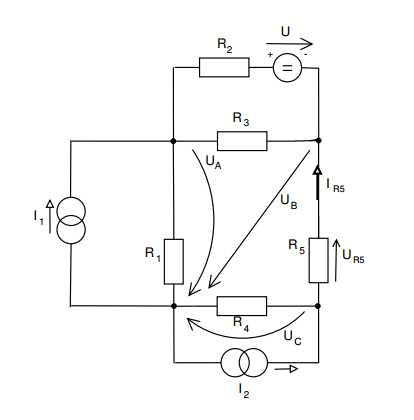
\includegraphics[width=10cm,keepaspectratio]{Napeti_3.PNG}
		\end{center}
	\end{figure}

	Napěťový zdroj převedeme na proudový:
	\begin{eqnarray*}
		I_{3} & = & U || R_{2} = \frac{U}{R_{2}} = \frac{130}{39} = 3.333\overline{3}A \\
	\end{eqnarray*}

	Zapíšeme v podobě rozšířené matice pomocí vodivosti:
	\begin{eqnarray*}
		A & = &
			\begin{pmatrix}			
				G_{1} + G_{2} + G_{3} & -G_{2} -G_{3} & 0 & \vline & I_{1} + I_{3} \\
				-G_{2} -G_{3} & G_{2} + G_{3} + G_{5} & -G_{5} & \vline & -I_{3} \\
				0 & -G_{5} &G_{4} + G_{5}& \vline & I_{2} \\
			\end{pmatrix} \\
		\\
		\Delta A & = &
			\begin{vmatrix}
				0.0642 & -0.0429 & 0 \\
				-0.0429 & 0.0829 & -0.04 \\
				0 & -0.04 & 0.0757 \\
			\end{vmatrix} = 0.0002 
	\end{eqnarray*}

	Budeme potřebovat matici pro $\Delta$B a $\Delta$C:
	\begin{eqnarray*}
		\Delta B & = & 
			\begin{vmatrix}
				0.0642 &  4.283\overline{3} & 0 \\
				-0.0429 & -3.333\overline{3} & -0.04 \\
				0 & 0.5 & 0.0757 \\
			\end{vmatrix} = -0.0010 \\
		\\
		\Delta C & = &
			\begin{vmatrix}
				0.0642 & -0.0429 & 4.283\overline{3} \\
				-0.0429 & 0.0829 & -3.333\overline{3} \\
				0 & -0.04 & 0.5 \\
			\end{vmatrix} = 0.0005 \\
	\end{eqnarray*}
	
	Pomocí Cramerova pravidla zjistíme napětí:
	\begin{eqnarray*}
		U_{B} & = & \frac{\Delta B}{\Delta A} = -\frac{-0.00100303}{0.00016073} = -6.2404V \\ 
		\\
		U_{C} & = & \frac{\Delta C}{\Delta A} = \frac{0.000531553}{0.00016073} = 3.3100V \\
	\end{eqnarray*}

	Výsledná rovnice pro zjištění $U_{R5}$ a $I_{R5}$:
	\begin{eqnarray*}
		U_{B} & = & U_{R4} + U_{R5} \\
		-U_{R} & = & -U_{B} - U_{R} = -6.2404 - 3.3100 = -9.5504V \\
		I_{R5} & = & \frac{U_{R5}}{R_{5}} = \frac{9.5504}{25} = 0.3818A\\
	\end{eqnarray*}

	Výsledek $U_{R5}$ a $I_{R5}$:
	\begin{eqnarray*}
		U_{R5} & = & 9.5504V \\
		I_{R5} & = & 0.3818A \\
	\end{eqnarray*}

%%%%%%%%%%%%%%%%%%%%%%%%%
%			CTVRTY PRIKLAD			   %
%%%%%%%%%%%%%%%%%%%%%%%%%

	\newpage
	\section{Smyčkové proudy v RLC obvodu}

	Pro napájecí napětí platí: $u_{1} = U_{1}\cdot sin(2\pi ft), u_{2} = U_{2}\cdot sin(2\pi ft)$. \\
	Ve vztahu pro napětí $u_{C1} = U_{C1}\cdot sin(2\pi ft + \phi_{C1})$ určete $|U_{C1}|$ a $\phi_{C1}$. Použijte metodu smyčkových proudů.\\
	\\
	Pozn: Pomocné "směry šipek napájecích zdrojů platí pro speciální časový okamžik $(t = \frac{\pi}{2\omega})$"

	\begin{table}[h]
		\begin{center}
			\begin{tabular}{|c|c|c|c|c|c|c|c|c|c|c|}
				\hline
				sk. & $U_{1}$ [$V$] & $U_{2}$ [$V$] & $R_{1}$ [$\Omega$] & $R_{2}$ [$\Omega$] & $R_{3}$ [$\Omega$] & $L_{1}$ [$mH$] & $L_{2}$ [$mH$] & $C_{1}$ [$\mu F$] & $C_{2}$ [$\mu F$] & $f$ [$Hz$]\\
				\hline
				B &  25 & 40 & 11 & 15 & 12 & 100 & 85 & 220 & 95 & 80 \\
				\hline
			\end{tabular}
		\end{center}
	\end{table}

	\begin{figure}[h]
		\begin{center}
			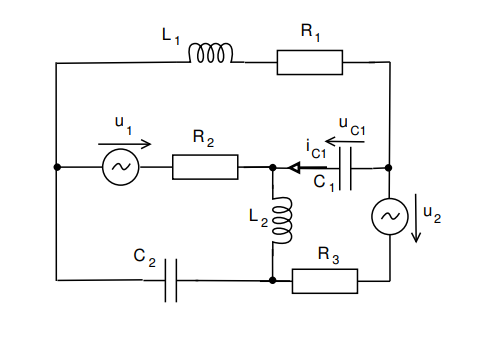
\includegraphics[width=12cm,keepaspectratio]{RLC_4.PNG}
		\end{center}
	\end{figure}

	Vypočteme impedance pro dané kondenzátory a cívky včetně $\omega$:
	\begin{eqnarray*}
		\omega & = & 2\pi f = 2\pi \cdot 80 = 502.6548 rad\cdot s^{-1} \\
		Z_{L1} & = & j \omega L_{1} = 502.6548  \cdot  100 \cdot 10^{-3} j = 50.2655 j \Omega \\
		Z_{L2} & = & j \omega L_{2} = 502.6548  \cdot  85 \cdot 10^{-3} j = 42.7257 j \Omega \\
		Z_{C1} & = & - \frac{1}{\omega C_{1}}j = - \frac{1}{502.6548 \cdot 220 \cdot 10^{-6}}j = -9.0429 j \Omega \\
		Z_{C2} & = & - \frac{1}{\omega C_{2}}j = - \frac{1}{502.6548  \cdot 95 \cdot 10^{-6}}j = -20.9414 j \Omega 
	\end{eqnarray*}

	Zavedeme smyčkové proudy $I_{A}, I_{B}, I_{C}$ a k nim příslušné rovnice:
	\begin{eqnarray*}
		Z_{L1} \cdot I_{A} + R_{1} \cdot I_{A} + Z_{C1} \cdot (I_{A} + I_{C}) + R_{2} \cdot (I_{A} - I_{B}) - U_{1} & = & 0 \\
		R_{2} \cdot (I_{B} - I_{A}) + Z_{L2} \cdot (I_{B} + I_{C}) + Z_{C2} \cdot I_{B} + U_{1} & = & 0 \\
		Z_{C1} \cdot (I_{C} + I_{A}) + Z_{L2} \cdot (I_{C} + I_{B}) + R_{3}  \cdot I_{C} - U_{2} & = & 0 \\
	\end{eqnarray*}

	Upravení rovnic:
	\begin{eqnarray*}
		I_{A} \cdot (Z_{L1} + R_{1} + Z_{C1} + R_{2}) - I_{B} \cdot R_{2} + I_{C} \cdot Z_{C1} & = & U_{1} \\
		-R_{2} \cdot I_{A} + I_{B} \cdot (R_{2} + Z_{L2} + Z_{C2}) + I_{C} \cdot Z_{L2} & = & -U_{1} \\
		I_{A} \cdot Z_{C1} + I_{B} \cdot Z_{L2} + I_{C} \cdot (Z_{C1} + Z_{L2} + R_{3}) & = & U_{2} \\
	\end{eqnarray*}

	Sestavení hlavní matice:
	\begin{eqnarray*}	
		\Delta A & = &
		\begin{vmatrix}
			26 + 41.2226j & -15 & -9.0428j \\
			-15 & 15 + 21.7842j & 42.7256j \\
			-9.0428j & 42.7256j & 12 + 33.6828j \\ 
		\end{vmatrix} =  -11602.7683 + 66559.4466j \\
	\end{eqnarray*}

	Sestavení matic pro výpočet $\Delta I_{C}$, $\Delta I_{A}$:
	\begin{eqnarray*}
		\Delta I_{A} =
		\begin{vmatrix}
			25 & -15 & -9.0428j \\
			-25 & 15 + 21.7842j & 42.7256j \\
			40 & 42.7256j & 12 + 33.6828j \\ 
		\end{vmatrix} =  9754.5181 - 13674.4200j \\
		\\
		\Delta I_{C} =
		\begin{vmatrix}
			26 + 41.2226j & -15 & 25 \\
			-15 & 15 + 21.7842j & -25 \\
			-9.0428j & 42.7256j & 40 \\ 
		\end{vmatrix} = -78276.3166 + 59138.6680j \\
	\end{eqnarray*}

	Výpočet proudů pomocí Cramerova pravidla:
	\begin{eqnarray*}
		I_{A} & = & \frac{\Delta I_{A}}{\Delta A} = -0.2242 - 0.1075jA \\
		I_{C} & = & \frac{\Delta I_{C}}{\Delta A} = 1.0613 + 0.9910jA \\
		I_{C1} & = & I_{A} + I_{C} = 0.8371 + 0.8835jA \\
	\end{eqnarray*}

	Napětí na $U_{C}$:
	\begin{eqnarray*}
	 	U_{C}  & = & I_{C1} \cdot Z_{C1} = (0.8371 + 0.8835j) \cdot (-9.0429j) = 7.9894 - 7.5698j \\
	\end{eqnarray*}

	Výsledek pro $|U_{C1}|$ a $\phi_{C1}$:
	\begin{eqnarray*}
		|U_{C}| & = & \sqrt{(imgU_{C})^2 + (realU_{C})^2} = \sqrt{7.5698^2 + 7.9894^2} = 11.0060V \\
		\phi_{C} & = & arctg(\frac{imgU_{C}}{realU_{C}}) = arctg(\frac{-7.5698}{7.9894}) = -0.7584 rad \\
	\end{eqnarray*}

%%%%%%%%%%%%%%%%%%%%%%%%%
%			PATY PRIKLAD			   %
%%%%%%%%%%%%%%%%%%%%%%%%%

	\newpage
	\section{Diferenciální rovnice}

	Sestavte diferenciální rovnici popisující chování obvodu na obrázku, dále ji upravte dosazením hodnot parametrů. Vypočítejte analytické řešení $u_{C} = f(t)$. \\
	Proveďte kontrolu výpočtů dosazením do sestavené diferenciální rovnice.
	\begin{table}[h]
		\begin{center}
			\begin{tabular}{|c|c|c|c|c|}
				\hline
				sk. & $U$ [$V$] & $C$ [$F$] & $R$ [$\Omega$] & $u_{C}(0)$ [$V$] \\
				\hline
				B &  40 & 10 & 20 & 8 \\
				\hline
			\end{tabular}
		\end{center}
	\end{table}
	\begin{figure}[h]
		\begin{center}
			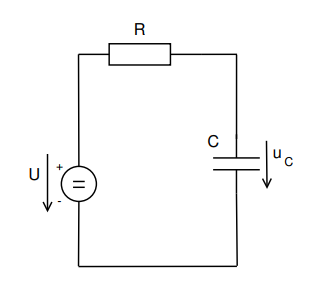
\includegraphics[width=8cm,keepaspectratio]{Diferencialni_5.PNG}
		\end{center}
	\end{figure}

	Podle \RN{2}. Kirchhoffova zákona sestavíme rovnici pro napětí ve smyčce, popisující proud:
	\begin{eqnarray*}
		0 & = & u_{R} + u_{C} - u \\
		0 & = & R \cdot I + u_{C} - u \\
		I & = & \frac{u - u_{c}}{R} \\
	\end{eqnarray*}

	Známe hodnoty můžeme dosadit do axiomu, který platí pro tento obvod:
	\begin{eqnarray*}
		u'_{C} & = & \frac{1}{C} \cdot I \\
		u'_{C} & = & \frac{u - u_{C}}{R \cdot C} \\
		u'_{C} & = & \frac{40 - u_{C}}{10 \cdot 20} \\
		u'_{C} & = & \frac{40}{200} - \frac{u_{C}}{200} \\
		\frac{1}{5} & = & u'_{C} + \frac{u_{C}}{200} \\
	\end{eqnarray*}
	
	Obecný tvar: 
	\begin{eqnarray*}
		u_{C}(t) & = & k(t)e^{\lambda t} \\
	\end{eqnarray*}

	Vypočteme si potřebnou $\lambda$:
	\begin{eqnarray*}
		\lambda + \frac{1}{200} & = & 0 \\
		\lambda & = & -\frac{1}{200} \\
	\end{eqnarray*}

	Nyní máme všechny potřebné hodnoty pro derivaci:
	\begin{eqnarray*}
		u_{C}(t) & = & k(t)e^{-\frac{1}{200}t} \\
		u'_{C}(t) & = & k'(t)e^{-\frac{1}{200}t} - \frac{1}{200} \cdot k(t)e^{-\frac{1}{200}t} \\
	\end{eqnarray*}

	Dané hodnoty dosadíme do rovnice obvodu:
	\begin{eqnarray*}
		 \frac{1}{5} & = & u'_{C} + \frac{u_{C}}{200} \\ \\
		 \frac{1}{5} & = & k'(t)e^{-\frac{1}{200}t} - \frac{1}{200} \cdot k(t)e^{-\frac{1}{200}t} +  \frac{1}{200} \cdot k(t)e^{-\frac{1}{200}t} \\ \\
		 \frac{1}{5} & = & k'(t)e^{-\frac{1}{200}t} \\
	\end{eqnarray*}

	Vyjádříme $k(t)$:
	\begin{eqnarray*}
		k'(t)e^{-\frac{1}{200}t} & = & \frac{1}{5} \\
		k'(t) & = & \frac{e^{\frac{1}{200}t}}{5} \\ 
		\int k'(t)dt & = & \frac{e^{\frac{1}{200}t}}{5} \\
		k(t) & = & 40e^{\frac{1}{200}t} + A \\
	\end{eqnarray*}

	Dosadíme hodnoty do obecného tvaru rovnice:
	\begin{eqnarray*}
		u_{C}(t) & = & k(t)e^{\lambda t} \\
		u_{C}(t) & = & (40e^{\frac{1}{200}t} + A) \cdot e^{-\frac{1}{200}t} \\
		u_{C}(t) & = & 40 + Ae^{-\frac{1}{200}t} \\
	\end{eqnarray*}

	Vliv počáteční podmínky:
	\begin{eqnarray*}
		u_{C}(0) & = & 40 + Ae^{-\frac{1}{200} \cdot 0 } \\
		8 & = & 40 + A \\
		A & = & -32 \\
	\end{eqnarray*}

	Hledaná rovnice tedy je: 
	\begin{eqnarray*}
		u_{C}(t) & = & 40 - 32e^{-\frac{1}{200}t} \\
	\end{eqnarray*}

	Kontrola:
	\begin{eqnarray*}
		u'_{C} + \frac{u_{C}}{200} & = & \frac{1}{5} \\
		u_{C}(t) & = & 40 - 32e^{-\frac{1}{5}t} \\
		u'_{c}(t) & = & \frac{32}{200}e^{-\frac{1}{5}t} \\
		\frac{1}{5} & = & \frac{32}{200}e^{-\frac{1}{200}t} + \frac{40 - 32e^{-\frac{1}{200}t}}{200} \\ \\
		\frac{1}{5} & = & \frac{1}{5} \\
	\end{eqnarray*}

	\newpage
	\section{Výsledková tabulka}
	\begin{table}[ht]
		\begin{center}
			\begin{tabular}{|c|c|c|}
				\hline
				Úloha & Skupina & Výsledky \\
				\hline
				\RN{1}. & B & $U_{R1} = 67.2812V$, $I_{R1} =  0.1035A$ \\
				\hline
				\RN{2}. & B & $U_{R3} = 36.7500 V$, $I_{R3} = 0.1670A$ \\
				\hline
				\RN{3}. & H & $U_{R5} = 9.5504 V$, $I_{R5} = 0.3818A$ \\
				\hline
				\RN{4}. & B & $|U_{C1}| = 11.0060 V$, $\phi_{C1} = -0.7584 rad$ \\
				\hline
				\RN{5}. &  B & $U_{c}(t) = 40 - 32e^{-\frac{1}{200} t}$ \\
				\hline
			\end{tabular}
		\end{center}
	\end{table}
\end{document}